\section{O Problema}

O desenvolvimento de um algoritmo evolutivo genérico para solucionar problemas com gamificação de disputas, ou seja, soluções que podem ser qualificadas entre o quão melhores uma é em relação as demais.

Estudar as aplicações desse algoritmo em um sistema com entradas e saídas bem definidas, de modo que a solução não esteja implícita em nenhuma das entradas e saídas, mas que o algoritmo possa evoluir livremente para encontrar o melhor rearranjo dos genes até produzir respostas idênticas as oferecidas pelo sistema.

\section{Biblioteca de Algoritmos Evolutivos}

Foi feita uma biblioteca para uso de algoritmos evolutivos em Java que empregas os conceitos de Indivíduos e Genes. Para aplicações diferentes das estudadas nesse documento, a biblioteca ainda pode ser usada em qualquer \SE, pois pode ser estendida e rearranjada para qualquer aplicação dentro desse conceito. As classes e métodos implementadas pela biblioteca estão descritas a seguir.

\subsection{Classe AE}

Esta classe é responsável por englobar as funções referentes ao algoritmo evolutivo em si, ou seja, ela organiza e remaneja os indivíduos, ela realiza confrontos, compara soluções, seleciona os melhores e recombina os indivíduos de modo que as melhores soluções propaguem suas características.

As disputas realizadas pelos indivíduos seguem um sistema de disputa mata-mata, que por padrão possui 16 participantes, onde o primeiro e segundo colocados propagam suas característica genética com os indivíduos que não foram enfrentados por eles. A Figura \ref{figura:funcao_playAll} demonstra visualmente como funciona esse torneio e a propagação das características dos melhores colocados.

% TODO: trocar figura e algoritmo pela função playAll
\begin{figure}[htb]
    \caption{Tornei realizado pela classe AE.}
    \label{figura:funcao_playAll}
    \centering
    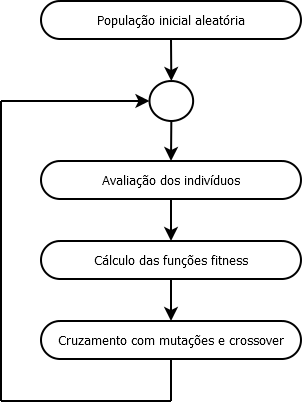
\includegraphics[scale=1]{images/dia/fluxograma-ae}
    \fautor
\end{figure}

A classe AE possui outras funções implementadas que são de uso diverso e serão discutidas em outra subseção.

\subsection{Classe Eq}

\newcommand{\var}[1]{\textit{#1}}

A classe Eq representa uma equação e possui uma função como representa a equação \ref{eq:eq}. Onde as variáveis \var{factor} e \var{sum} correspondem a variáveis internas da classe.

\begin{equation}
    \label{eq:eq}
    f(x)=\mathrm{factor}*x + \mathrm{sum}
\end{equation}

\subsection{Classe Indivíduo}

A classe indivíduo representa um indivíduo capaz de gerar uma solução para o sistema. A função \fitness é responsável por informar se um indivíduo ganhará um confronto de outro, quanto maior a função \fitness, melhor.

Na biblioteca, o indivíduo possui o método \method{play} que recebe outro indivíduo como parâmetro. O usuário escolhe como confrontar os dois indivíduos retornando 0 se o vencedor for indivíduo que chama o método, ou 1, se o vencedor for o indivíduo referenciado no parâmetro. Nesta função não é possível retornar uma informação para os casos de empate. Como este projeto foca uma disputa entre dois indivíduos, o método \method{play} pode confrontar esses dois indivíduos $N$ vezes e basear sua função \fitness com base nas partidas vencidas, além de retornar o indivíduo que mais venceu partidas como vitorioso.

\subsection{Classe Gene}

Cada indivíduo pode possuir uma determinada quantidade de genes que são capazes de gerar uma resposta. O gene pode ser excitado de alguma forma pelo sistema e possui um valor de estado que pode aumentar de acordo com a operação operação de consumir um estado. Portanto um gene possui duas funções que envolvem a variável \var{estado}:

\begin{itemize}
    \item \method{Consumir}: O método de \method{consumir} altera a variável \var{estado} do gene conforme a equação \ref{eq:gene_consumir} onde $x$ é o valor da entrada, $i$ é a posição da entrada no ventor de entradas de um sistema, ou seja, se um sistema possui entradas com vetor de tamanho $N$, $i$ terá valores de 0 até $N-1$, $E$ e $I$ são funções descritas em \ref{eq:eq}.
    \begin{equation}
        \label{eq:gene_consumir}
        \mathrm{Estado} \leftarrow \mathrm{Estado} +  E(x) * I_i(i)
    \end{equation}
    \item \method{Reset}: O método de \method{reset} devolve o \var{estado} do gene para um estado inicial. A classe Gene possui as variáveis internas \var{estado}, \var{estadoInicial}, \var{limiteSup} e \var{limiteInf}. A função de \method{reset} está descrita no algoritmo \ref{algoritmo:gene_reset}.
\end{itemize}

\begin{algoritmo}
\caption{Algoritmo de reinicio de gene.}
\label{algoritmo:gene_reset}
    \If(\tcp*[f]{Se o estado do gene está fora dos limites})
    {estado > limiteSup {\normalfont \textbf{or}} estado < limiteInf} {
        $estado \gets estadoInicial$
    }
\end{algoritmo}

\subsection{Outras implementações}

A biblioteca implementa outras funções que são necessárias para a execução do \SE e facilitam o trabalho de desenvolvedores que usam a biblioteca, elas são:

\begin{itemize}
    \item Funções para gerar números aleatórios:
        \begin{itemize}
            \item Funções para gerar números aleatórios inteiros ou com ponto decimal;
            \item Função para gerar números aleatórios com desvio-padrão deslocado para as bordas, pois a solução pode ter uma combinação de valores bem distinta.
        \end{itemize}
    \item Cruzamento de números: esta função realiza um sorteio com as possibilidades de:
        \begin{itemize}
            \item Manter o valor que estava;
            \item Adquirir o valor da melhor solução;
            \item Definir o novo valor como a média entre a melhor solução e o valor atual.
        \end{itemize}
    \item Uma classe de estados: como esse projeto tem uma área dedicada ao estudo de previsão de estados, a classe de estados implementada para essa solução foi mantida no projeto de biblioteca para um \SE.
    \item Descarte dos piores genes: a fim de aumentar a variabilidade genética, há um parâmetro que configura o número de gerações para que ocorra um descarte dos piores indivíduos por novos.
\end{itemize}

Esse conjunto de funções extra torna o uso da biblioteca em outros projetos como um aumento de produtividade e diminuição do tempo necessário para a conclusão.

\subsection{Resultados}

A biblioteca produzida pode ser aplicada para quaisquer situações em que a gamificação baseada em disputas de dois jogadores pode ser aplicada. Por outro lado, essa biblioteca encara a função \fitness do algoritmo evolutivo de outra forma, o melhor algoritmo é aquele capaz de vencer mais jogos.

Outro fator importante para o sucesso da biblioteca é o fator de que os indivíduos que não foram confrontados são aqueles que recebem os as característica do melhor. Assim, cria-se a lógica de que as estratégias tomadas por um dos indivíduos passará para o outro ramo de jogadores. A Figura \ref{figura:ae_torneio_passos} mostra como essa estratégia da biblioteca funciona.

% TODO: trocar figura
\begin{figure}[htb]
    \caption{Demonstração de passos do torneio.}
    \label{figura:ae_torneio_passos}
    \centering
    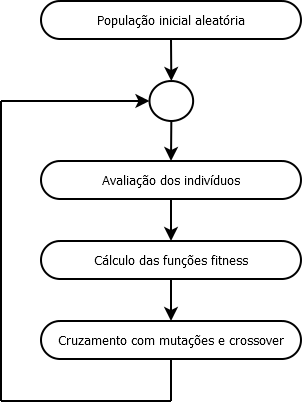
\includegraphics[scale=1]{images/dia/fluxograma-ae}
    \fautor
\end{figure}

A biblioteca facilita o desenvolvimento de programas que necessitam de um \SE por já estar implementada e testada. Qualquer usuário pode reutilizar a biblioteca, pois ela é de código aberto e está disponibilizada através da plataforma GitHub\footnote{Disponível em \url{https://github.com/}}. Além disso, a biblioteca implementa alguns conceitos no \SE que guiam o pensamento do desenvolvedor.

\section{Algoritmo evolutivo para previsão de estados}

Foi feito um estudo utilizando a biblioteca desenvolvida nesse projeto a fim de criar um sistema que recebe um vetor de Estado e é capaz de prever os resultados dos estados de saída baseado nas entradas.

O vetor de estados é uma classe que possui um vetor de entradas e um vetor de saídas, mas as saídas são bem definidas, ou seja, seguem um número limitado que vai de 0 até $N-1$, sendo o $N$ o número de saídas possíveis.

Para esse projeto, foi feito um estudos com saídas de tamanho $N=3$, um número relativamente pequeno, mas que pode representar muitas situações, como casos de uma previsão de vitória, derrota ou empate. Além disso, um número de saída pequeno diminui o tempo de convergência do algoritmo evolutivo, permitindo que vários testes possam ocorrer e várias alterações de melhorias puderam ser tomadas durante o tempo de produção desse projeto.

A biblioteca produzida foi estendida e utilizada, as alterações feitas para o uso da biblioteca estão detalhadas a seguir.

\subsection{Classe Indivíduo}

Um indivíduo é recebe as entradas do sistema e a cada iteração, produz uma saída de acordo com os valores de estado de seus genes. Um bom individuo é aquele capaz de prever as saídas dos estados dependendo das entradas. O melhor indivíduo é aquele que prevê todas saídas.

Os confrontos entre indivíduos se dão do seguinte critério:
\begin{itemize}
    \item Comparação entre o número de acertos: os indivíduos que mais acertaram estados de saídas são considerados melhores do que indivíduos que acertaram menos.
    \item Comparação entre a segunda hipótese de saída: os indivíduos que não acertaram o estado, mas que deixaram a saída correta como segunda opção ficam melhores posicionados do que os indivíduos que também não acertaram, mas que também não consideraram a saída correta como segunda hipótese.
\end{itemize}

Paralelamente, os indivíduos possuem uma função de pontuação que aumenta em 1 quando um indivíduo acerta uma resposta como primeira alternativa, e aumenta em 0,5 quando um indivíduo acerta a resposta como segunda alternativa.

\subsection{Classe Resposta de Gene}

Essa classe é uma extensão da classe Gene, acrescentando as seguintes funcionalidades:
\begin{itemize}
    \item Conter mais genes consecutivos: cada gene forma uma lista encadeada com outro gene.
    \item Cada gene possui uma informação de resposta: as respostas possíveis de cada gene variam de 0 até $N-1$.
\end{itemize}

Mas essa classe segue as mesmas regras da classe Gene, ou seja, o Gene mais excitado é considerado como a resposta do indivíduo.

\subsection{Estados do sistema analisados}

Entre os possíveis estados para se analisar, a melhor escolha foi um sistema de vetor de entradas $E$ de tamanho 3 e vetor de saídas $S$ de tamanho 1 descrito por:

\begin{gather*}
    2 \quad \mathrm{se} \quad E_3 > E_1 \quad \mathbf{e} \quad E_3 > E_2 \\
    1 \quad \mathrm{se} \quad \sum E_2 > \sum E_1 \\
    0 \quad \mathrm{c.c.}
\end{gather*}

Esse sistema é um bom caso de estudo pois:

\begin{itemize}
    \item Possui fatores acumulativos: a resposta do sistema depende de uma memória, ou seja, o estado anterior influencia na próxima resposta.
    \item Possui fatores situacionais: a resposta do sistema depende de uma situação momentânea, ou seja, para determinadas entradas, a resposta descarta uma lógica.
    \item Possui muitas comparações: o sistema faz várias comparações e o algoritmo evolutivo deve imitar ou simular as comparações para obter as respostas.
\end{itemize}

Os valores de entrada foram obtidos aleatoriamente e foram feitos teste com 200 e 100 estados, mas o há uma condição, o número de saídas de um valor de resposta deve ser de no mínimo um quinto do número de estados, isso foi determinado para que houvesse uma quantidade razoável de todas as respostas possíveis. Testes com 200 estados produziram resultados semelhantes aos teste com 100 estados, porém o algoritmo necessita de mais tempo para convergir, por isso, o daremos foco com testes de 100 estados.

\subsection{Resultados}

Os resultados variam de acordo com a amostragem, porém as taxas de acerto obtida pelo algoritmo foram melhores do que tentativas aleatórias.

O conjunto 1 de estados produziu uma resposta com taxa de acerto de 96 dentre os 100 e 97,5 pontos. Nesse caso, o indivíduo com melhor resposta possui 4 genes, 2 genes destinas a resposta 2 e as demais respostas com apenas 1 gene. Para esse mesmo conjunto de estados, mas com obtenção de genes aleatórios, o melhor indivíduo encontrado após o mesmo número de gerações obteve 72 acertos com 84,5 pontos. A convergência do algoritmo ocorreu aproximadamente com 50.000 gerações. A Figura \ref{figura:resultado_97} mostra a evolução da função \fitness.

% TODO: trocar figura
\begin{figure}[htb]
    \caption{Histórico de \fitness do conjunto 1 de estados.}
    \label{figura:resultado_97}
    \centering
    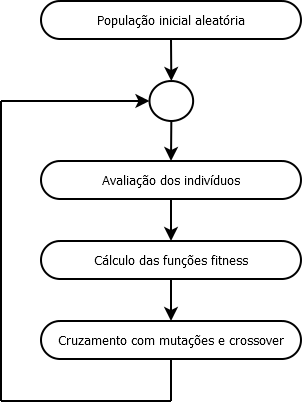
\includegraphics[scale=1]{images/dia/fluxograma-ae}
    \fautor
\end{figure}

Outro conjunto 2 de estados obteve uma resposta com taxa de acerto de 79 de 100 e 86,5 pontos. Nesse caso, o indivíduo com melhor resposta possui 4 genes, 2 genes destinas a resposta 0 e as demais respostas com apenas 1 gene. Apesar desse conjunto ter uma resposta muito inferior ao conjunto 1, ainda assim, o algoritmo evolutivo foi melhor do que uma tentativa de genes aleatórios, que obtiveram 77 acertos com 84 pontos. Ambos os resultados foram obtidos com aproximadamente 70.000 gerações. A Figura \ref{figura:resultado_79} mostra a evolução da função \fitness.

% TODO: trocar figura
\begin{figure}[htb]
    \caption{Histórico de \fitness do conjunto 2 de estados.}
    \label{figura:resultado_79}
    \centering
    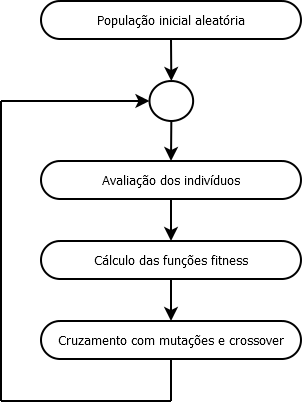
\includegraphics[scale=1]{images/dia/fluxograma-ae}
    \fautor
\end{figure}

\section{Dificuldades e Limitações}

\subsection{Sobre a biblioteca desenvolvida}

A biblioteca está bem implementada e testada, entretanto, limita o usuário a linguagem Java. Idealmente a biblioteca deveria ser escrita em C/C++, compilada como executável de biblioteca dinâmica e adaptada para as mais diversas linguagens do mercado, essas mudanças ajudariam no desempenho e no reuso da biblioteca para outras linguagens. O projeto não foi desenvolvido dessa maneira pelas vantagens citadas na seção \ref{secao:rev_bib}, por se tratar de um material de estudo, os benefícios de Java foram importantes para o projetista.

\subsection{Sobre o algoritmo evolutivo para previsão de estados}

Os testes aplicados a esse estudos obtiveram resultados melhores do que vetores aleatórios, mas se demonstraram dependentes dos valores fornecidos. Em situações com uma amostragem de dados muito grande, é possível selecionar os melhores dados para alimentar o algoritmo evolutivo a fim de se encontrar os melhores parâmetros para previsão.

O testes realizados foram com poucas entradas e com poucas saídas definidas, devido ao tempo computacional requerido para muitas entradas ou muitas saídas.
